\documentclass{beamer}
\usetheme{Singapore}
\usecolortheme{crane}
\usepackage{iwona}
\usepackage{graphicx}
\usepackage{amsmath}
\usepackage{mathdots}
\usepackage{amsthm}
\usepackage{amssymb}
\usepackage{hyperref}
\usepackage{lscape}
\usenavigationsymbolstemplate{}
\def\insertnavigation#1{\relax}

\title{Week 0}
\author{Geraint Palmer\\Room: M/1.29\\\url{palmergi1@cardiff.ac.uk}\\}
\date{\tiny{Last updated \today}}

\begin{document}

\maketitle

\frame{\frametitle{Overview}\tableofcontents}

\section{Algebra}

\frame{
  \frametitle{Algebra}
  Wikipedia:\\
  \vspace{.5cm}
  ``Algebra is the branch of mathematics concerning the study of the rules of
  operations and relations, and the constructions and concepts arising from
  them, including terms, polynomials, equations and algebraic structures.''
}


\subsection{Numbers}

\frame{
  \frametitle{Numbers}
  \begin{itemize}
    \item Integers: $$\mathbb{Z} = \{\dots, -3, -2, -1, 0, 1, 2, 3, \dots\}$$
    \item Rationals:
    $$\mathbb{Q} = \left\{ a \nonscript\; | \nonscript\; \exists \nonscript\; p, q \in \mathbb{Z} \text{ for which } a = {p \over q}\right\}$$
    \item Real numbers: $$\mathbb{Z} \subset \mathbb{Q} \subset \mathbb{R}$$
  \end{itemize}
}


\subsection{Exponents}

\frame{
  \frametitle{Exponents}
  If $a$ and $b$ are any positive real numbers and $x$ and $y$ are any real
  numbers then:
  \begin{enumerate}
    \item $a^x a^y = a^{x+y}$
    \item $a^0 = 1$
    \item $a^{-x} = {1 \over a^x}$
    \item $\left(a^x\right)^y = a^{xy}$
    \item $a^x b^x = (ab)^x$
  \end{enumerate}
}


\subsection{Inequalities}

\frame{
  \frametitle{Inequalities}
  When solving inequalities it is important to keep in mind whether or not the
  operation we are using is an \emph{increasing} or a  \emph{decreasing} one.
  \begin{center}
    \includegraphics[width=4.5cm]{increasing_plot.pdf}\hspace{1cm}
    \includegraphics[width=4.5cm]{decreasing_plot.pdf}\\
    $a < b\Rightarrow f(a) < f(b)$ \hspace{2.5cm} $a < b \Rightarrow g(a) > g(b)$
  \end{center}
}


\subsection{Graphs}

\frame{
  \frametitle{Coordinates in the plane}
  The location of a point in a plane can be specified in terms of right handed
  cartesian axes:
  \begin{center}
    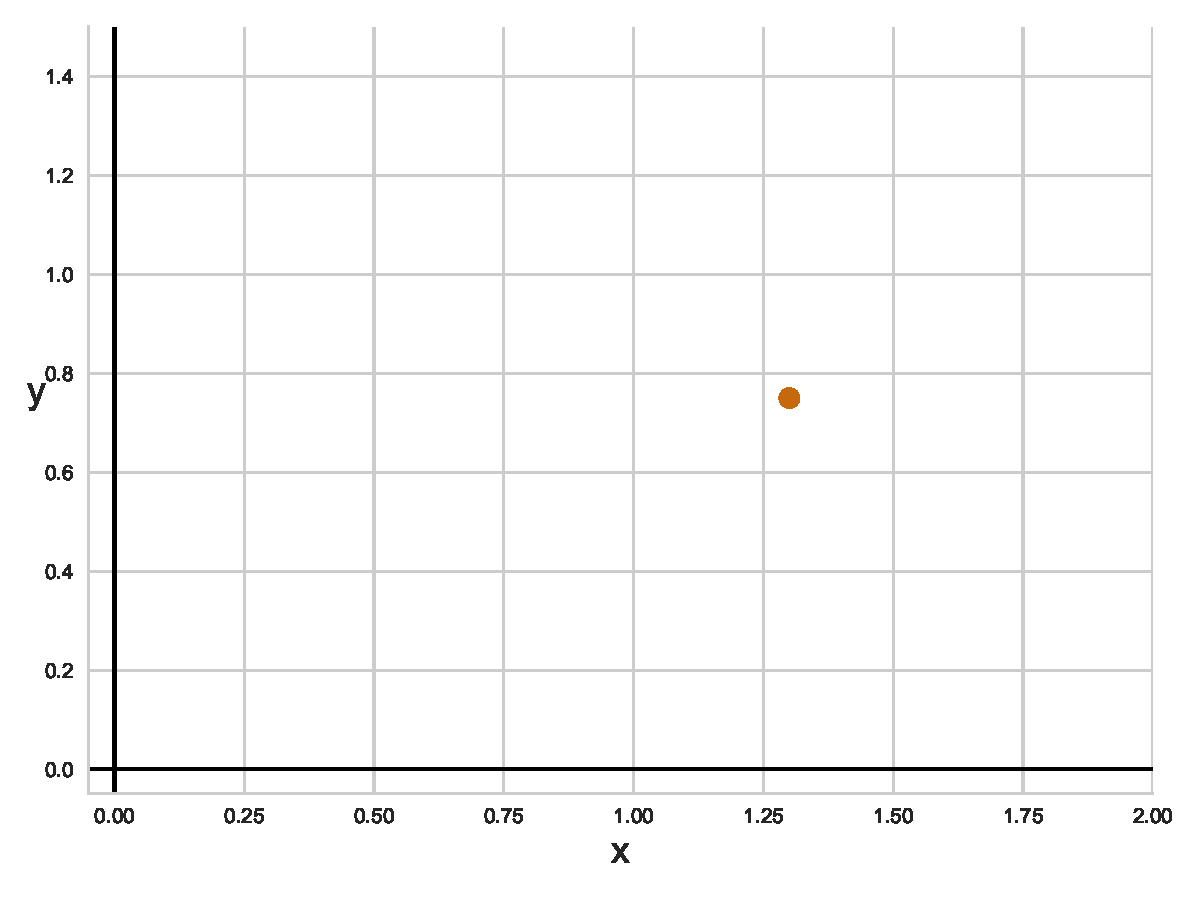
\includegraphics[width=7cm]{coordinate_system}
  \end{center}
  The point $(1.3, 0.75)$ is plotted above.\\
  In general for a point $P = (x, y)$, $x/y$ is called the abscissa/ordinate of
  $P$.
}

\frame{
  \frametitle{Graphs}
  If $x$ and $y$ connected by an equation, then this relation can be represented
  by a curve or curves in the $(x, y)$ plane which is known as the graph of the
  equation.
  \begin{center}
    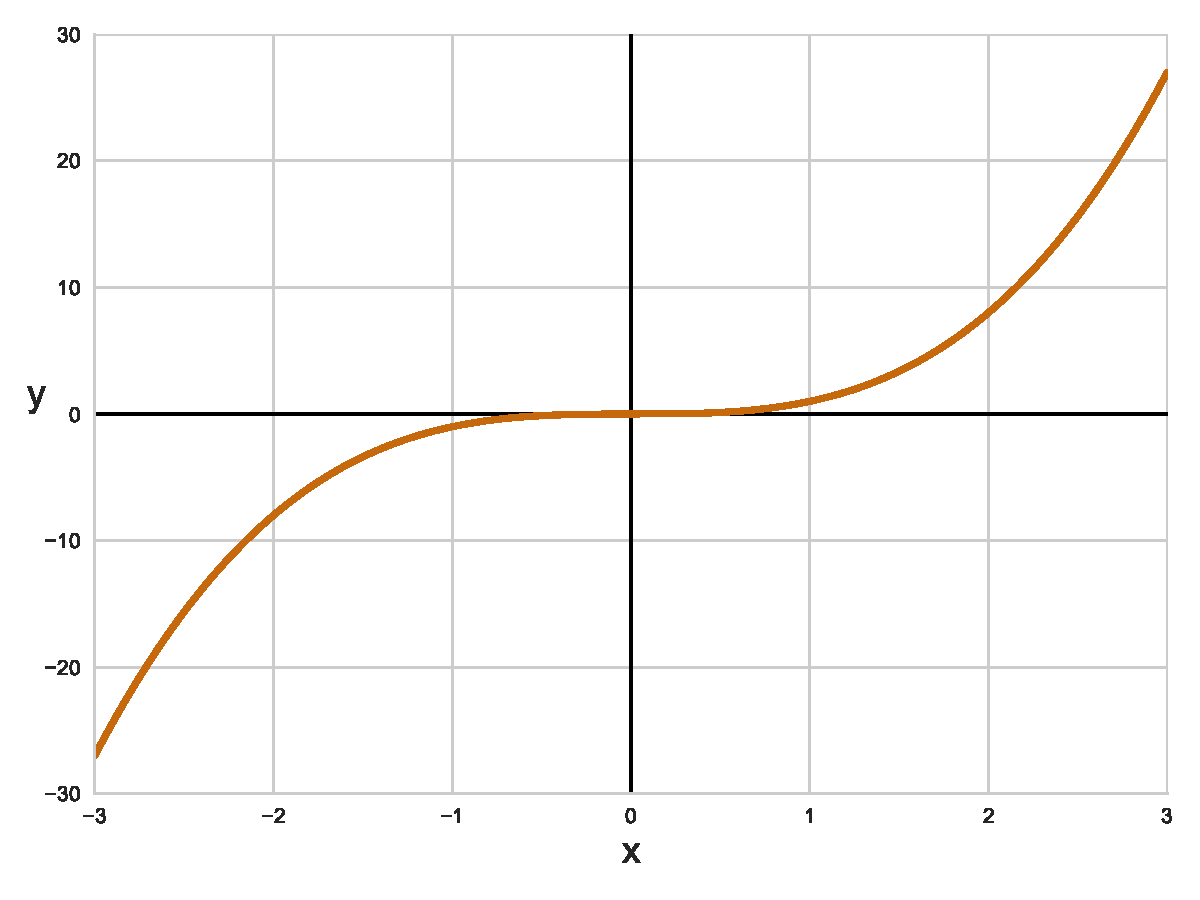
\includegraphics[width=7cm]{xcubed}
  \end{center}
  The equation $y = x^3$ is plotted above.
}


\frame{
  \frametitle{Graphs}
  One particular type of graph is the graph of a line: $$y = mx + b$$
  \begin{itemize}
    \item $m$ is called the \emph{gradient} of the line.
    \item $b$ is called the $y$\emph{-intercept} of the line.
  \end{itemize}
}

\frame{
  \frametitle{Exercise}
  Find the equation for the line going through the points $\{(0.5, 3),(4, 1.1)\}$:
  \begin{center}
    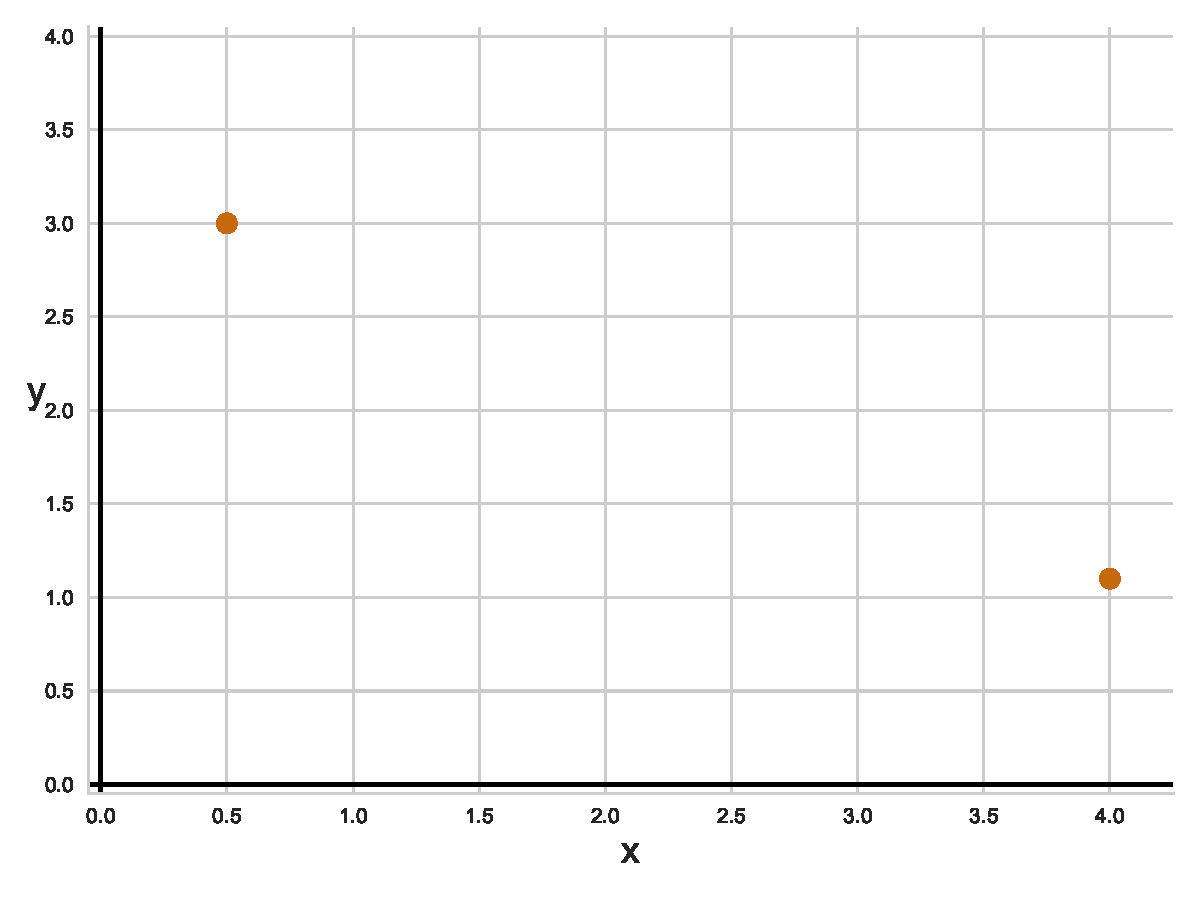
\includegraphics[width=7cm]{2points}
  \end{center}
}

\frame{
  \frametitle{Solution}
  General form of line $y=mx+b$ through $\{(x_1, y_1),(x_2, y_2)\}$ can be
  obtained:
  $$\left.
    \begin{array}{@{}r@{\;}c@{\;}l@{}}
      y_1 & = & mx_1 + b\\
      y_2 & = & mx_2 + b
    \end{array}
  \right\}
  \Rightarrow
  \left.
    \begin{array}{@{}r@{\;}c@{\;}l@{}}
      m(x_1 - x_2) & = & y_1 - y_2\\
      c(a_2 - a_1) & = & a_2 b_1 - a_1 b_1
    \end{array}
  \right\}$$
  which gives:
  $$\begin{array}{@{}r@{\;}c@{\;}l@{}}
    m & = & {y_1 - y_2 \over x_1 - x_2}\\[2mm]
    c & = & {x_2 y_1 - x_1 y_2 \over x_2 - x_1}
  \end{array}$$
}

\frame{
  \frametitle{Solution}
  So for $(x_1, y_1)=(0.5, 3)$ and $(x_2, y_2)=(4, 1.1)$ we have:
  $$\begin{array}{@{}r@{\;}c@{\;}l@{}}
    m & = & {1.9 \over -3.5} \approx -0.54\\[2mm]
    c & = & {11.45 \over 3.5} \approx 3.27
  \end{array}$$
  \begin{center}
    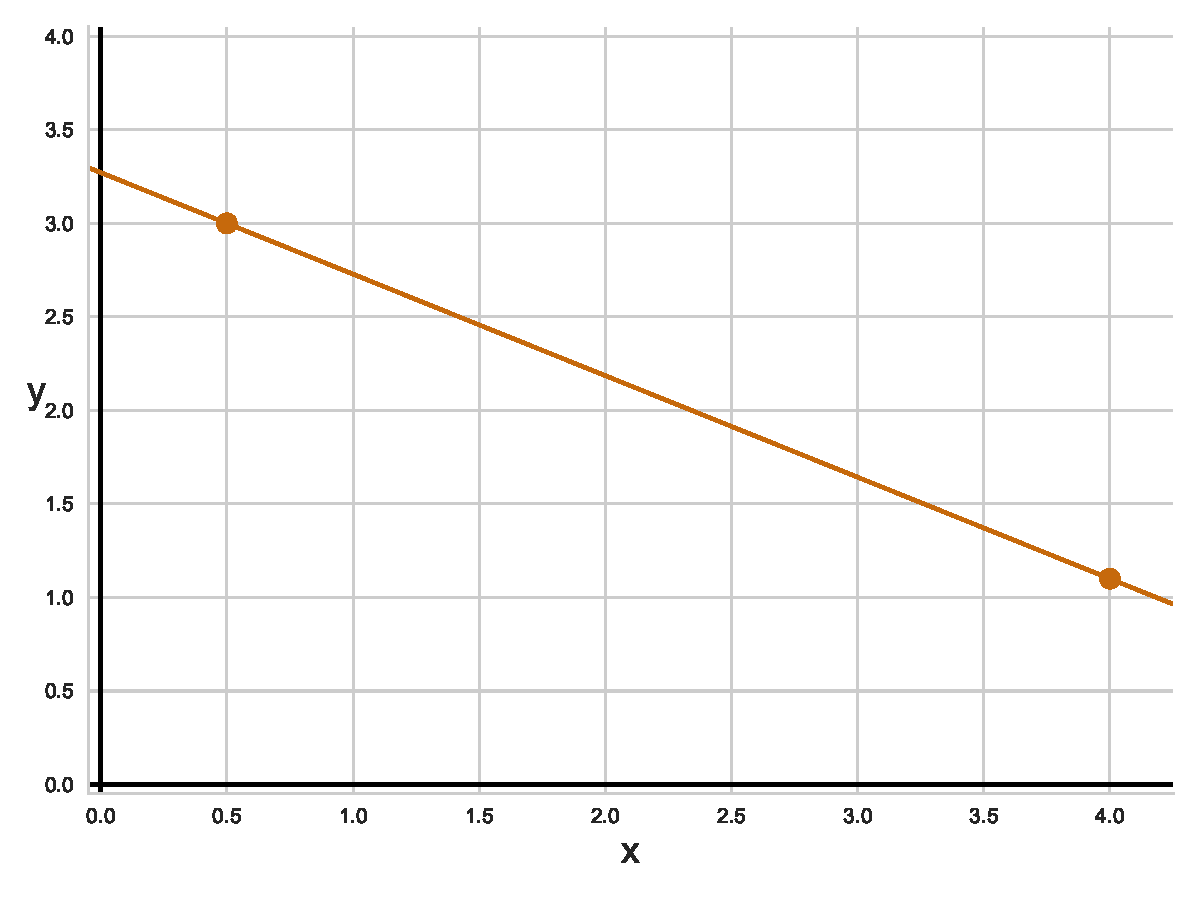
\includegraphics[width=7cm]{2pointsandline}
  \end{center}
}

\frame{
  \frametitle{Exercise}
  Where does the line $y = -0.54x + 3.27$ intersect the $y$-axis and the $x$-axis?\\
  \pause
  This is equivalent to solving:
  $$y = -0.54 \times 0 + 3.27$$
  and
  $$0 = -0.54x + 3.27$$
}


\subsection{Linear Equations}

\frame{
  \frametitle{Solving Linear Equations}
  In general equations of the form:
  $$y=mx+b$$ are solved by muliplying or adding various constants.

  \begin{align*}
    0 = -0.54x + 3.27
      &\Leftrightarrow
    0 - 3.27 = (-0.54x + 3.27) - 3.27\\
    -3.27 = -0.54x
      &\Leftrightarrow
    -3.27 \times {1 \over -0.54} = 0.54x \times {1 \over -.54}\\
    x &\approx 6.06
  \end{align*}
}

\frame{
  \frametitle{Solving Linear Equations}
  In general equations of the form:
  $$y = mx + b$$ are solved by muliplying or adding various constants.
  
  \begin{align*}
    y = mx + b
      &\Leftrightarrow
    y - b = (mx + b) - b\\
    y - b = mx
      &\Leftrightarrow
    (y - b) \times {1 \over m} = mx \times {1 \over m}\\
    x &= {y - b \over m}
  \end{align*}
}


\subsection{Quadratic Equations}

\frame{
  \frametitle{Quadratic}A ``quadratic'' is an expression of the form:
  $$ax^2 + bx + c$$
  \begin{itemize}
    \item $a$ is called the quadratic coefficient,
    \item $b$ is called the linear coefficient,
    \item $c$ is called the constant term or free term.
  \end{itemize}
}

\frame{
  \frametitle{Quadratic}
  \begin{center}
    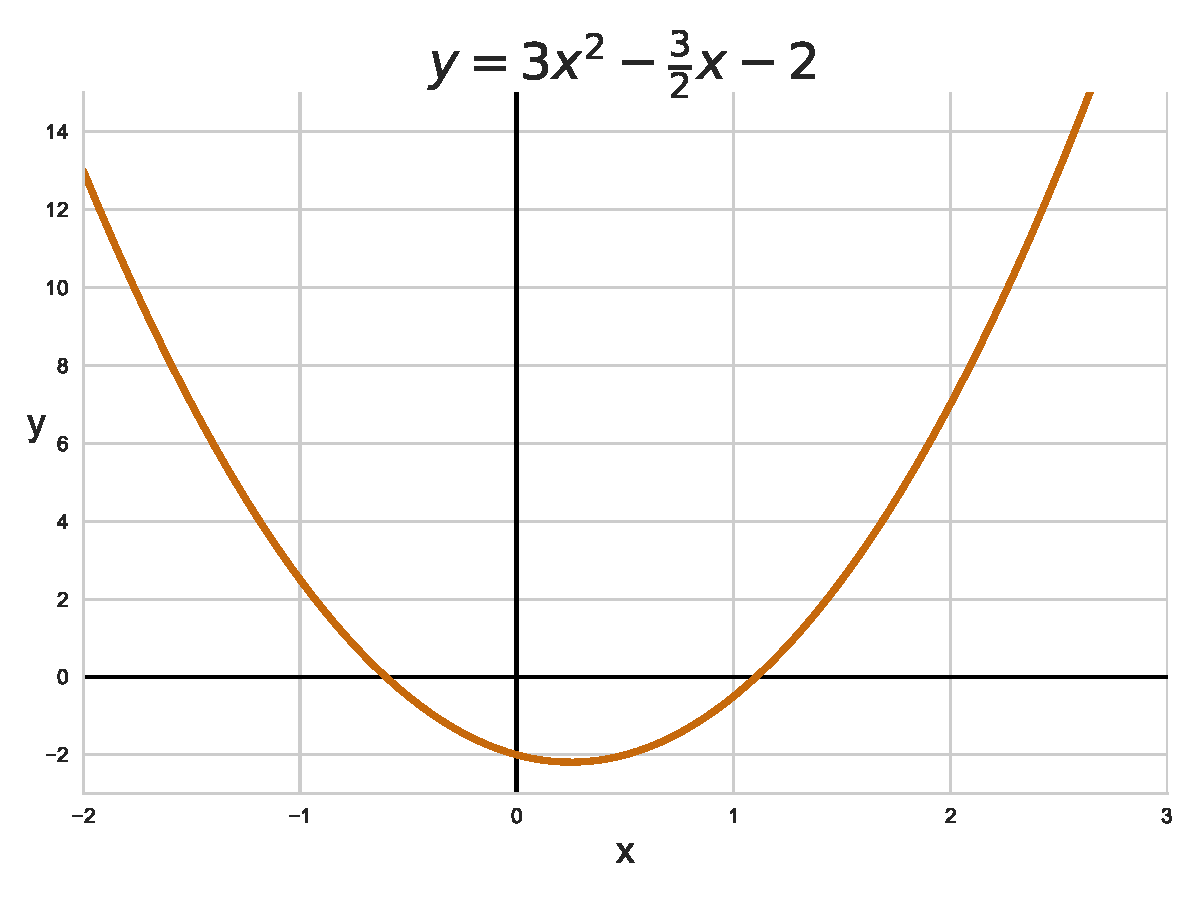
\includegraphics[width=7cm]{quadratic.png}
  \end{center}
}

\frame{
  \frametitle{Solving a Quadratic Equation}
  General solution of the equation:
  $$ax^2 + bx + c = 0$$
  is given by:
  $$x = {-b \pm \sqrt{b^2 - 4ac} \over 2a}$$
}

\frame{
  \frametitle{Exercise}
  Solve the equation:
  $$3x^2 - {3 \over 2} x - 2 = 0$$
}

\frame{
  \frametitle{Solution}
  From the previous formula we have:
  
  \begin{align*}
    x = {{3 \over 2} \pm \sqrt{\left({3 \over 2}\right)^2 - 4 \times 3 \times(-2)} \over 2 \times 3}
      &\Leftrightarrow
    x = {{3 \over 2} \pm \sqrt{{9 \over 4} + 24} \over 6}\\
    x = {3 \over 12} \pm {{1 \over 2} \sqrt{9 + 96} \over 6}
      &\Leftrightarrow
    x = {1 \over 4} \pm {\sqrt{105} \over 12}
  \end{align*}
}

\frame{
  \frametitle{Exercise}
  Solve the equation:
  $$4x^2 - 2x + 10 = 3$$
}

\frame{
  \frametitle{Solution}
  From the previous formula we have:

  \begin{align*}
    x = {2 \pm \sqrt{2^2 - 4 \times 4 \times 7} \over 2 \times 4}
      &\Leftrightarrow
    x = {2 \pm \sqrt{-108} \over 8}\\
    x = {2 \pm \sqrt{i^2108} \over 8}
      &\Leftrightarrow
    x = {2 \pm i\sqrt{3 \times 36} \over 8}\\
    x = {2 \pm 6i\sqrt{3}\over8}
      &=
    {1 \over 4} \pm {3 \over 4} i\sqrt{3}
\end{align*}
}


\subsection{Complex Numbers}

\frame{
  \frametitle{Very brief description of Complex Numbers}
  $$i^2 = -1$$
  Complex numbers:
  $$\mathbb{C} = \left\{a + bi \nonscript\; | \nonscript\; a, b \in \mathbb{R} \right\}$$
  If $z = a + ib$:
  \begin{itemize}
    \item $a$ is the real part of $z$.
    \item $b$ is the imaginary part of $z$.
  \end{itemize}
}


\subsection{Systems of Equations}

\frame{
  \frametitle{Solving Systems of Equations}
  A system of equations is a collection of equations involving the same set of
  variables. For example:

  \begin{align*}
    3x + 2y &= 1\\
    2x - 2y &= -2
  \end{align*}
Various techniques can be used to solve such a problem.
}

\frame{
  \frametitle{Elimination of Variables}
  \begin{itemize}
    \item Use first equation to obtain expression for first variable as a
    function of other variables.
    \item Substitute and use second equation to obtain expression for second
    variable as a function of other variables.
    \item etc...
  \end{itemize}
}

\frame{
  \frametitle{Exercise}
  Solve:

  \begin{align*}
    3x + 2y &= 1\\
    2x - 2y &= -2
  \end{align*}
}

\frame{
  \frametitle{Solution}
  First equation gives:
  $$3x + 2y = 1 \Rightarrow x = {1 - 2y \over 3}$$
  Substituting in to second equation gives:
  $$2\left(1 - 2y \over 3\right) - 2y = -2$$
  which implies:
  $$y = {4 \over 5}$$
  Substituting in to our expression for $x$ we get:
  $$x = -{1 \over5}$$
}


\subsection{Induction}

\frame{
  \frametitle{Shorthand notation}
  \begin{itemize}
    \item Summation: $$\sum_{i=1}^{n} a_i = a_1 + a_2 + a_3 + \dots + a_n$$
    \item Multiplication: $$\prod_{i=1}^{n} a_i = a_1 \times a_2 \times a_3 \times \dots \times a_n$$
  \end{itemize}
}

\frame{
  \frametitle{Examples}
  \begin{itemize}
    \item Summation: $$\sum_{i=1}^4 i \times 2^{i} = 1 \times 2 + 2 \times 2^2 + 3 \time 2^3 + 4\times 2^4 = 2 + 8 + 3 \times 8 + 4 \times 16 = 98$$
    \item Multiplication: $$\prod_{k=1}^3 k^{2} = 1 \times 2^2 \times 3^2 = 36$$
  \end{itemize}
}

\frame{
  \frametitle{Proof by Induction}
  Technique often used to prove algebraic relationships. Basic idea:
  \begin{itemize}
    \item Prove that something is true at the start.
    \item Prove that if something is true at point $k$ then it is true at point $k + 1$.
  \end{itemize}
  \only<1>{
    \begin{center}
      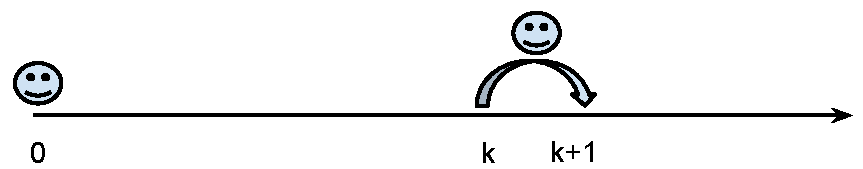
\includegraphics[width=7cm]{inductionpic}
    \end{center}
  }
  \only<2>{
    \begin{center}
      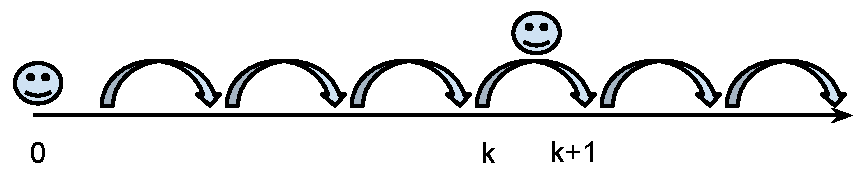
\includegraphics[width=7cm]{inductionpic1}
    \end{center}
  }
}

\frame{
  \frametitle{Exercise}
  Prove that: $$\sum_{i=0}^n i = {n(n + 1)\over 2}$$
}

\frame{
  \frametitle{Solution}
  \begin{itemize}
    \item True for $n = 0$?:
      $$\sum_{i=0}^0 i = 0 \text{ and }{n(n + 1) \over 2} = 0$$
    \item If true for $n=k$, true for $n=k+1$?:
      $$\sum_{i=0}^{k+1} i= \sum_{i=0}^{k} i + k + 1 ={k(k + 1) \over 2} + k + 1 = {(k + 1)(k + 2) \over 2}$$
  \end{itemize}
}


\section{Calculus}

\frame{
  \frametitle{Calculus}
  Wikipedia:\\\vspace{.5cm}
  ``Calculus is the study of change, in the same way that geometry is the study
  of shape and algebra is the study of operations and their application to
  solving equations''
}


\subsection{Functions}

\frame{
  \frametitle{Functions}
  A function $f$ is a rule that assigns to each element $x$ in a set $D$ exactly
  one element, called $f(x)$, in a set $E$.
  \pause
  \begin{center}
    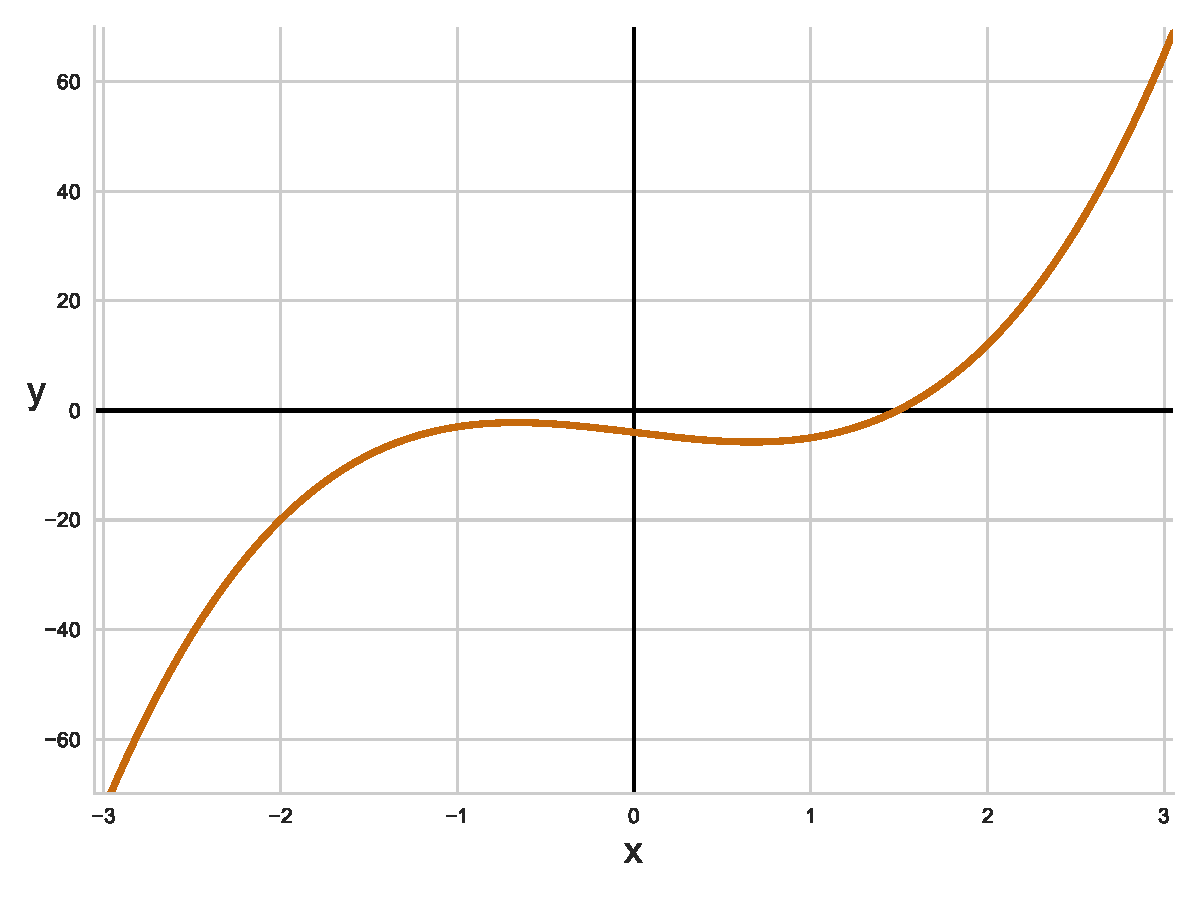
\includegraphics[width=7cm]{function}
  \end{center}
  \pause
  \begin{itemize}
    \item We usually consider functions for which the sets $D$ and $E$ are sets
    of real numbers.
    \item The set $D$ is called the domain of the function.
    \item The range of $f$ is the set of all possible values of $f(x)$ as $x$
    varies throughout the domain.
    \item A symbol that represents an arbitrary number in the domain of a
    function $f$ is call an independent variable.
    \item A symbol that represents a number in the range of $f$ is called a
    dependent variable.
  \end{itemize}
}

\frame{
  \frametitle{Example}
  The function $f(x) = 3x^3 - 4x - 4$ is plotted below:
  \begin{center}
    \includegraphics[width=7cm]{complicated_function}
  \end{center}
}

\frame{
  \frametitle{Even and Odd Functions}
  \begin{itemize}
    \item If a function $f$ satisfies $f(-x) = f(x)$ for all $x$ in its domain
    then $f$ is called an even function:
    \begin{center}
      \includegraphics[width=4cm]{even_function}
    \end{center}
    \item If a function $f$ satisfies $f(-x) = -f(x)$ for all $x$ in its domain
    then $f$ is called an odd function:
    \begin{center}
      \includegraphics[width=4cm]{odd_function}
    \end{center}
  \end{itemize}
}


\subsection{Differentiation}

\frame{
  \frametitle{Tangent Curves}
  The tangent line to the curve $y = f(x)$ at the point $P = (a, f(a))$ is the line
  through $P$ with gradient:
  $$m = \lim_{x \to a}{f(x) - f(a) \over {x - a}}$$
}

\frame{
  \frametitle{Tangent Curves}
  \only<1>{
    \begin{center}
      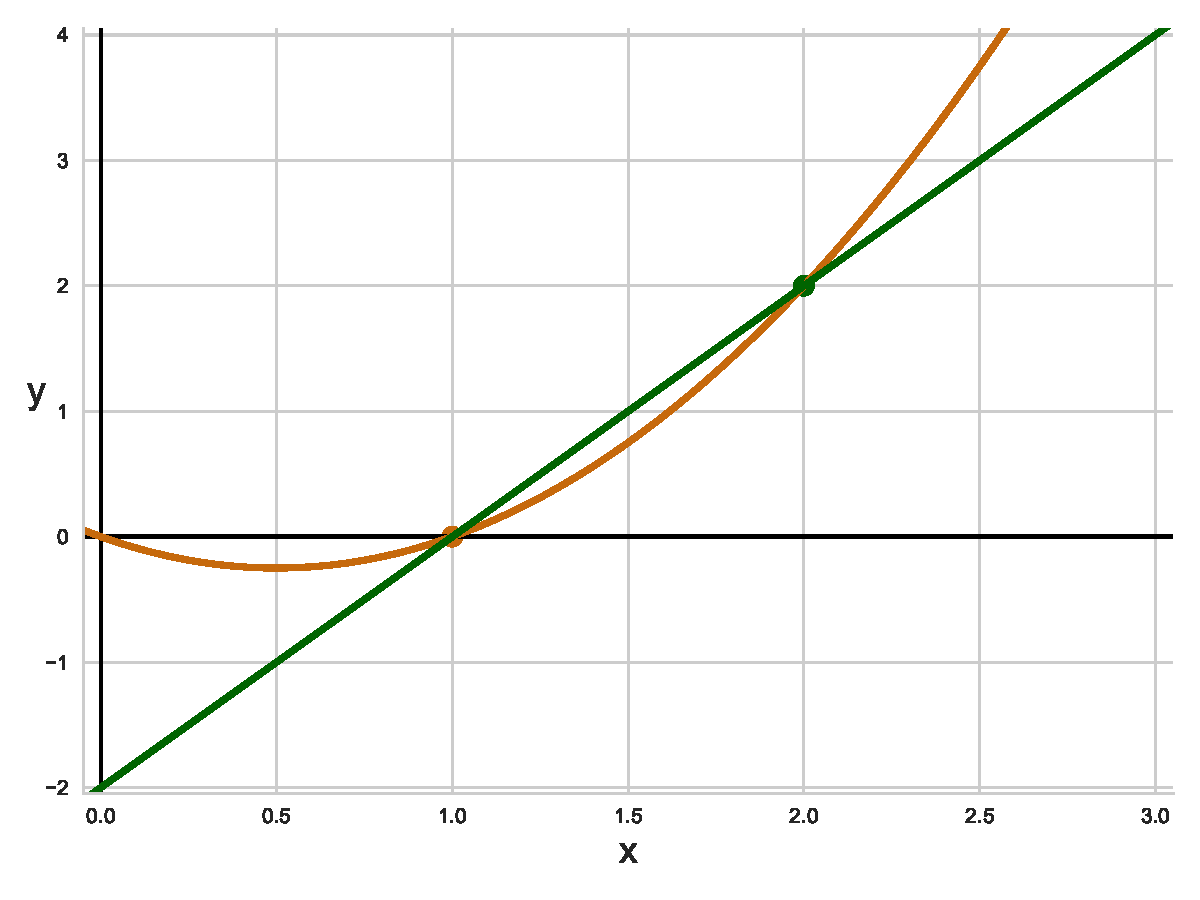
\includegraphics[width=7cm]{tangent_line}
    \end{center}
  }
  \only<2>{
    \begin{center}
      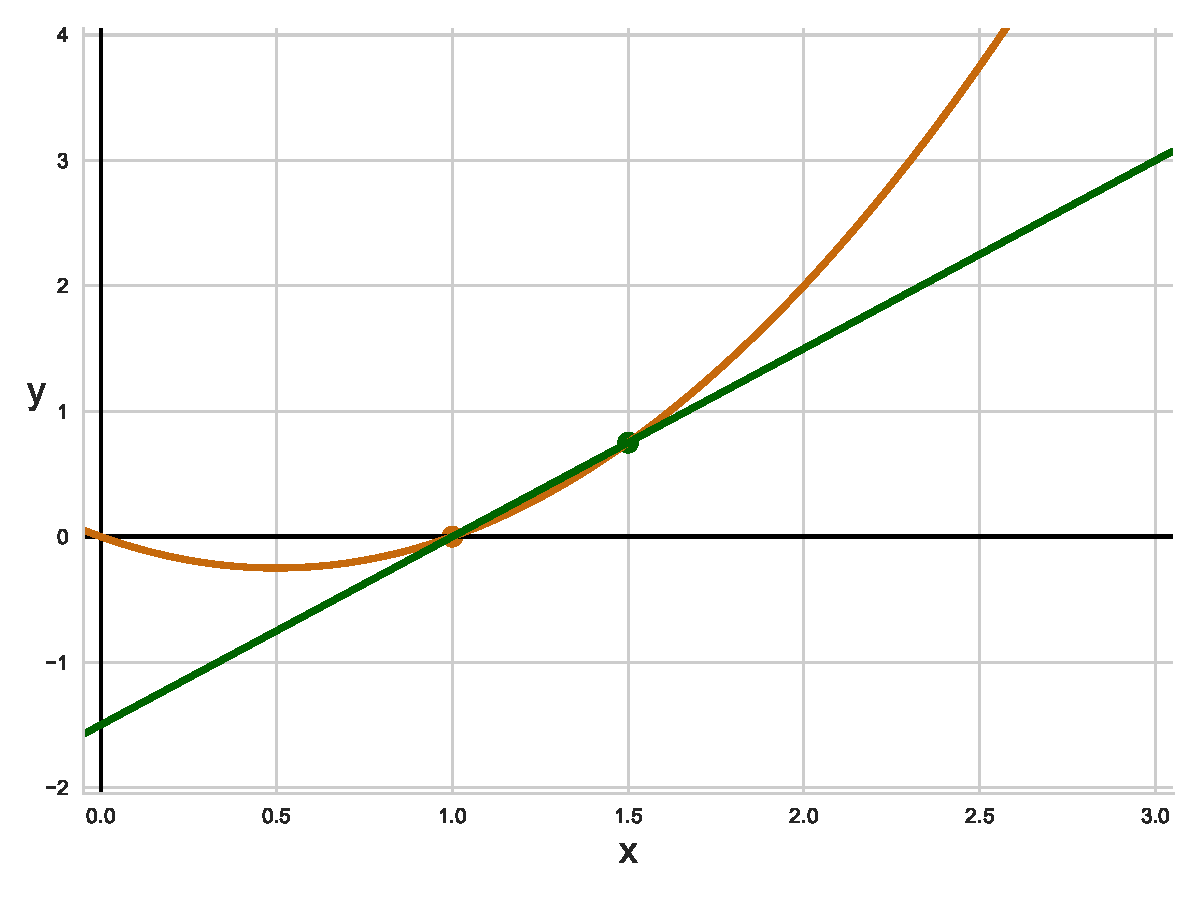
\includegraphics[width=7cm]{tangent_line_1}
    \end{center}
  }
  \only<3>{
    \begin{center}
      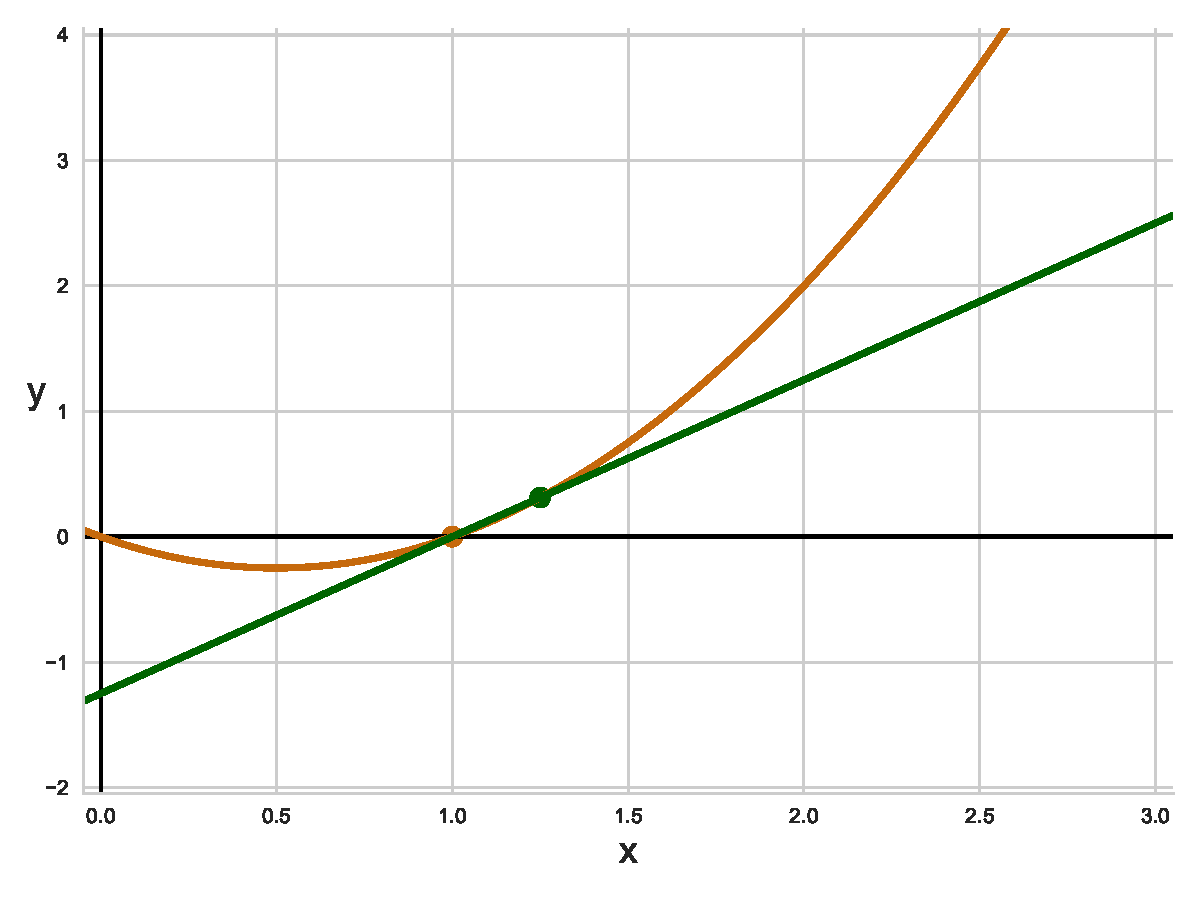
\includegraphics[width=7cm]{tangent_line_2}
    \end{center}
  }
  \only<4>{
    \begin{center}
      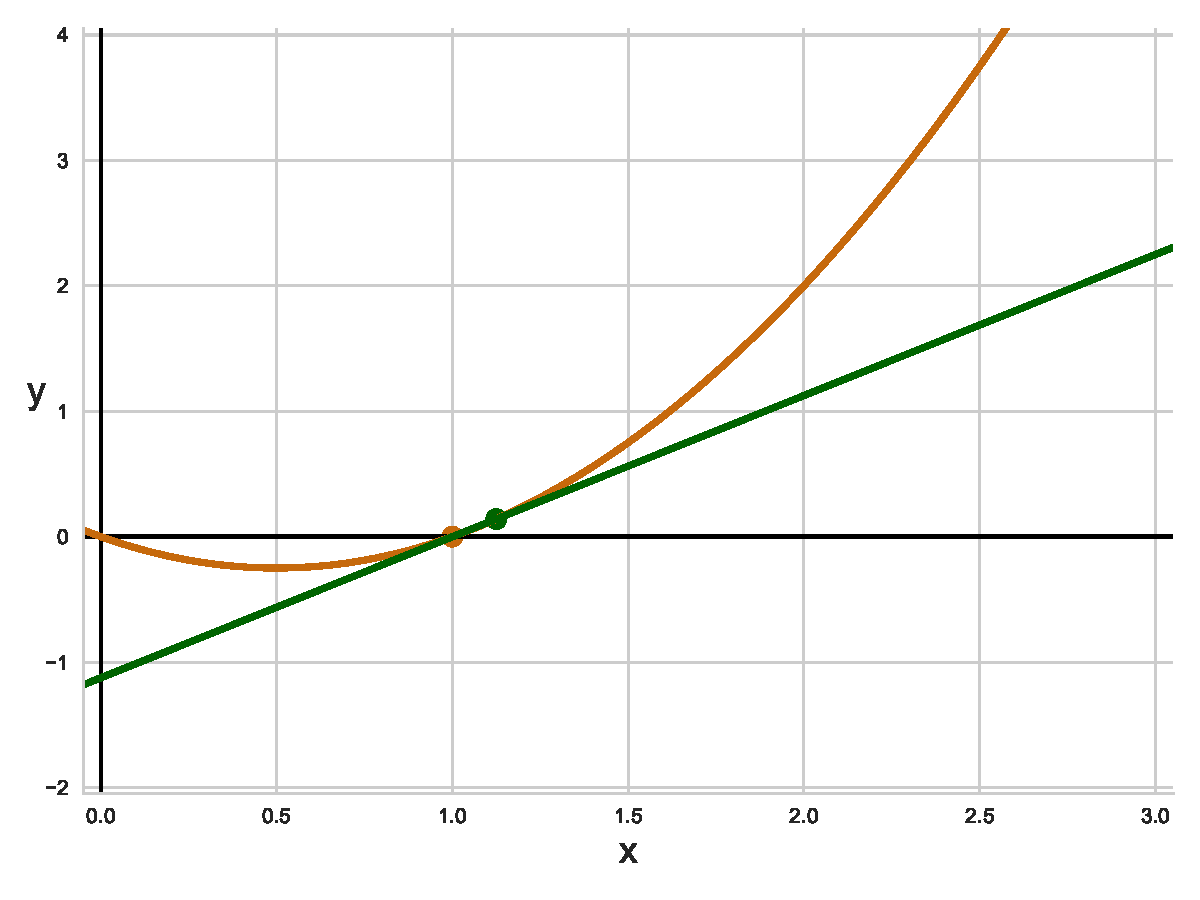
\includegraphics[width=7cm]{tangent_line_3}
    \end{center}
  }
  \only<5>{
    \begin{center}
      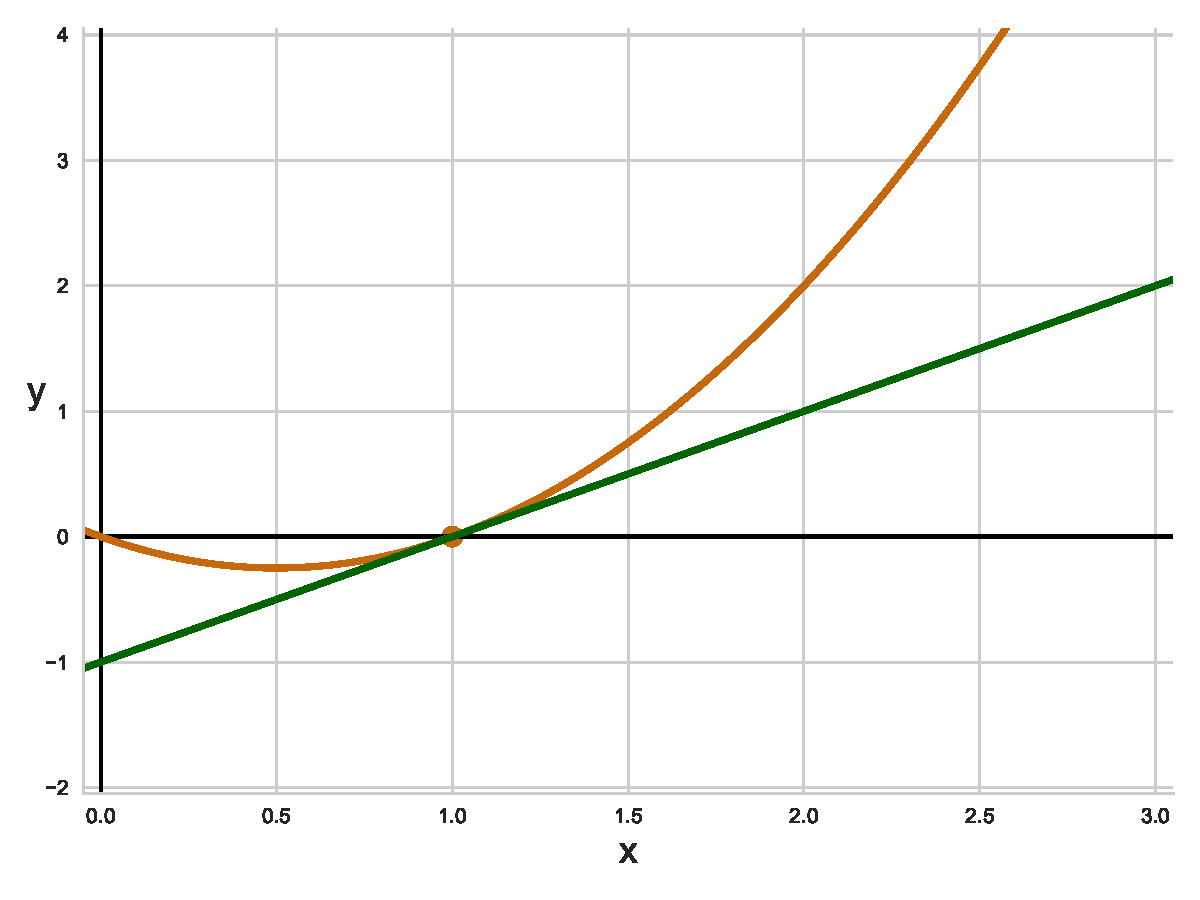
\includegraphics[width=7cm]{tangent_line_4}
    \end{center}
  }
}

\frame{
  \frametitle{Derivative}
    The derivative of a function $f$ at a number $a$, denoted by $f'(a)$ is:
    $$f'(a) = \lim_{h \to 0}{f(a + h) - f(a) \over h}$$
}

\frame{
  \frametitle{Exercise}
    Find the derivative of the function $f(x) = x^2 - 3x + 2$ at the number $a$.
}

\frame{
  \frametitle{Solution}
  \begin{align*}
    f'(a)
    &= \lim_{h \to 0}{f(a + h) - f(a) \over h}\\
    &= \lim_{h \to 0}{\left((a + h)^2 - 3(a + h) + 2 \right) - \left(a^2 - 3a + 2 \right) - f(a) \over h}\\
    &= \lim_{h \to 0}{a^2 + 2ah + h^2 - 3a - 3h + 2 - a^2 + 3a - 2 \over h}\\
    &= \lim_{h \to 0}{2ah + h^2 - 3h \over h}\\
    &= \lim_{h \to 0}{2a + h - 3}\\
    &= 2a - 3
  \end{align*}
}

\frame{
  \frametitle{Rules of Differentiation}
  \begin{itemize}
    \item The Power Rule:
    $${d \over dx}\left(x^n\right) = nx^{n - 1}$$
    \item The Constant Multiple Rule:
    $${d \over dx}\left(cf(x)\right) = c{d \over dx}\left(f(x)\right)$$
    \item The Sum Rule:
    $${d \over dx}\left(f(x) + g(x)\right) = {d \over dx}\left(f(x)\right) + {d \over dx}\left(g(x)\right)$$
\end{itemize}
}

\frame{
  \frametitle{Rules of Differentiation}
  \begin{itemize}
    \item The Product Rule:
    $${d \over dx}\left(f(x)g(x)\right) = g(x){d \over dx}\left(f(x)\right) + f(x){d \over dx}\left(g(x)\right)$$
    \item The Quotient Rule:
    $${d\ over dx}\left({f(x) \over g(x)}\right) = {g(x){d \over dx}\left(f(x)\right) - f(x){d \over dx}\left(g(x)\right) \over g(x)^2}$$
  \end{itemize}
}

\frame{
  \frametitle{The Chain Rule}
  If $g$ and $f$ are two functions with derivatives $g'$ and $f'$ respectively
  then:
  $${d \over dx}\left(f(g(x))\right) = f'(g(x))g'(x)$$
}

\frame{
  \frametitle{Exercise}
  Differentiate $F(x)=\sqrt{x^2 + 1}$.
}

\frame{
  \frametitle{Solution}
  If we let $f(x) = \sqrt{x}$ and $g(x) = x^2 + 1$ then we have:
  $${d \over dx}f(x)={d \over dx}x^{1 \over 2}={1 \over 2}x^{{1 \over 2} - 1} = {1 \over 2\sqrt{x}}\text{ and } {d \over dx}g(x) = 2x$$
  Using the Chain Rule we have:
   $${d \over dx}F(x)={1 \over 2\sqrt{x^2 + 1}} 2x = {x \over \sqrt{x^2 + 1}}$$
}


\frame{
  \frametitle{Natural Exponential Function}
  The mathematical constant $e$ can be defined as the real number such that:
  $${d \over dx}e^x = e^x$$
  \begin{center}
    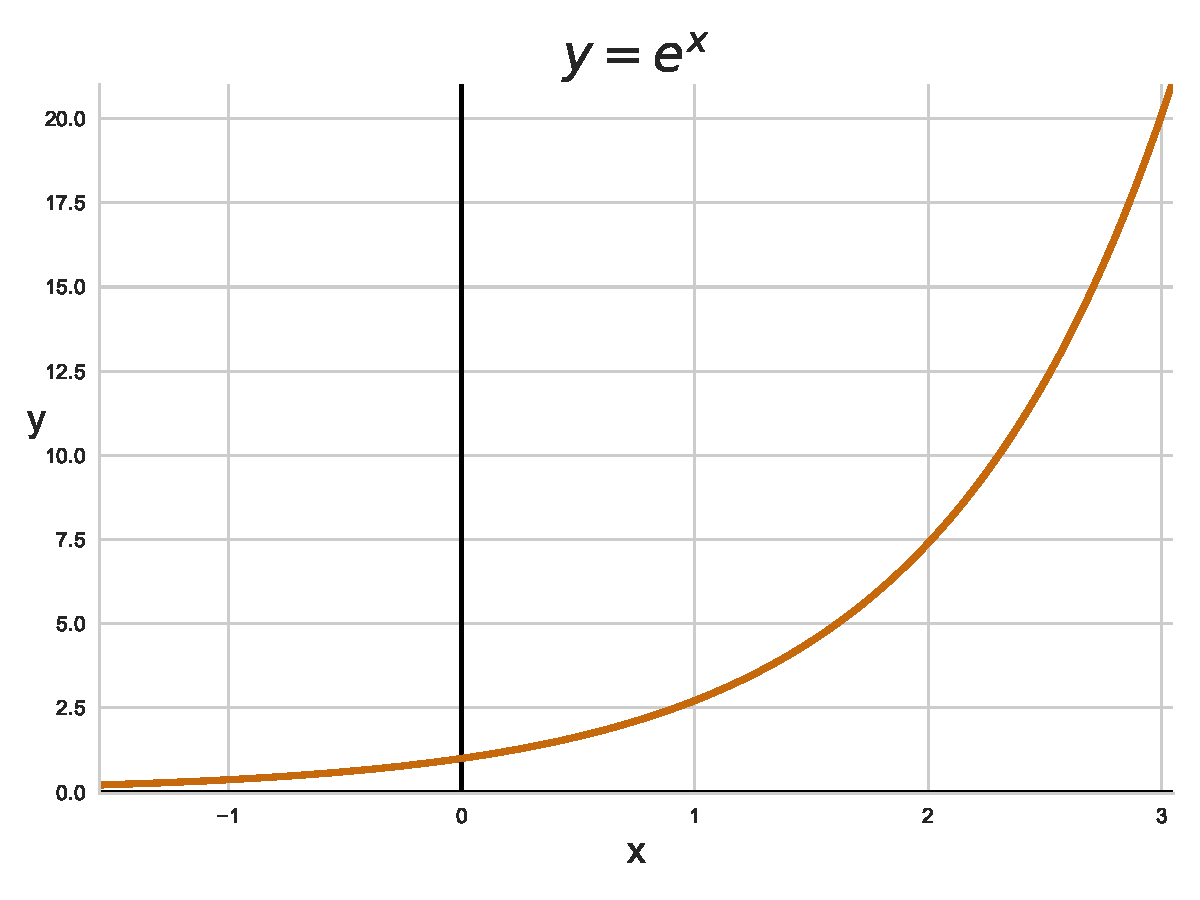
\includegraphics[width=7cm]{exp}
  \end{center}
}

\frame{
  \frametitle{Trigonometric Functions}
  $$\begin{array}{@{}l@{\;\;\;}l@{}}
    \displaystyle{{d \over dx}\sin(x) = \cos(x)} &
    \displaystyle{{d \over dx}\csc(x) = -\csc(x)\cot(x)}\\[3mm]
    \displaystyle{{d \over dx}\cos(x) = -\sin(x)}&
    \displaystyle{{d \over dx}\sec(x) = \sec(x)\tan(x)}\\[3mm]
    \displaystyle{{d \over dx}\tan(x) = \sec^2(x)}&
    \displaystyle{{d \over dx}\cot(x) = -\csc^2(x)}
  \end{array}$$
}


\subsection{Integration}

\frame{
  \frametitle{Area under a graph}
  \begin{center}
    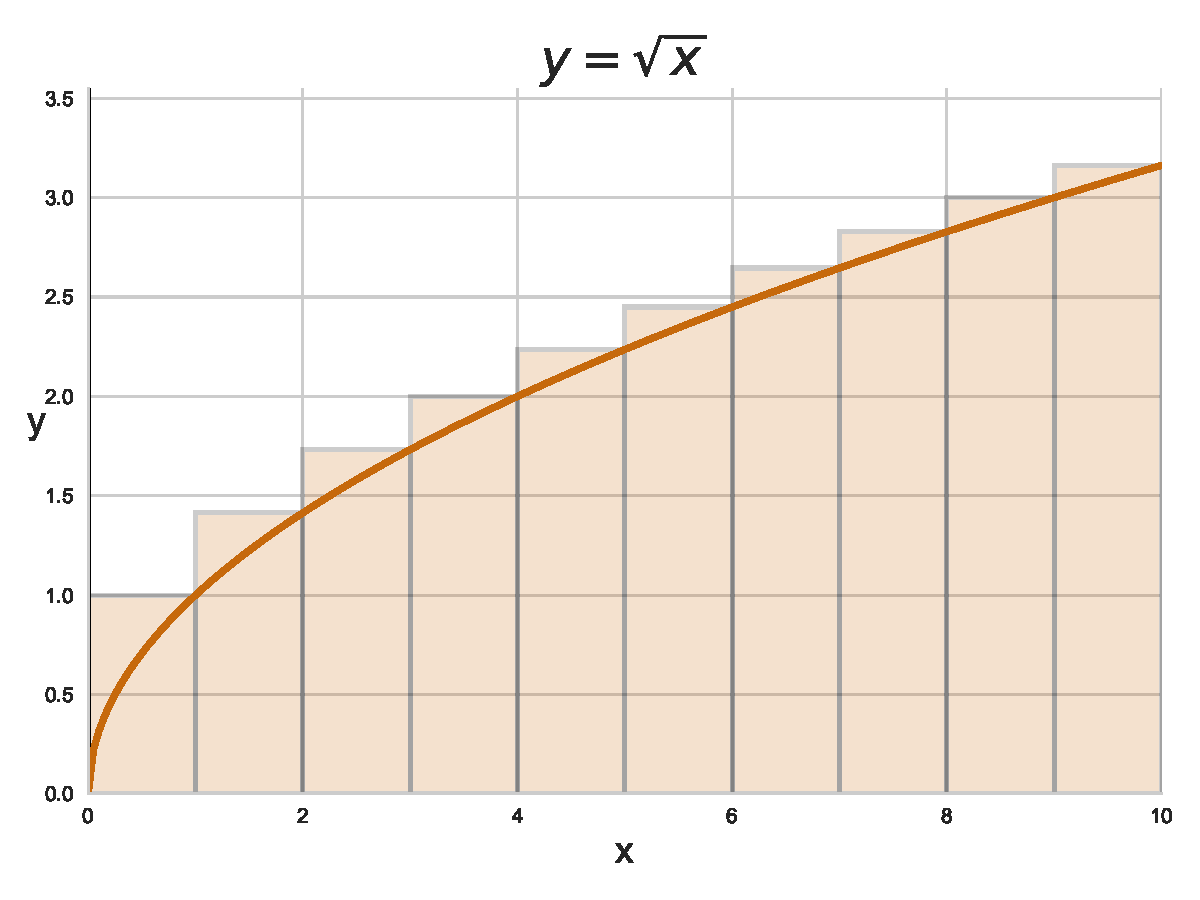
\includegraphics[width=7cm]{area_under_graph.pdf}
  \end{center}
}

\frame{
  \frametitle{Fundamental Theorem of Calculus}
  If $f$ is continuous on $[a,b]$ then:
  \begin{enumerate}
    \item If $g(x) = \int_{a}^x f(t)dt$ then ${d \over dx}g = f$.
    \item $\int_{a}^b f(x)dx = F(b) - F(a)$ where $F$ is any function such that
    ${d \over dx}F = f$.
\end{enumerate}}

\frame{
  \frametitle{Indefinite Integrals}
  $$\int f(x)dx = F(x)\text{ means }{d \over dx}F=f$$
}

\frame{
  \frametitle{Exercise}
  Calculate: $$\int{x^2 + \sin(x)dx}$$
}

\frame{
  \frametitle{Solution}
  Since ${d\ over dx}x^3 = 3x^2$ we have $\int{x^2 dx}={x^3 \over 3}$.
  Similarly, since ${d \over dx}\cos(x) = -\sin(x)$ we have:
  $$\int{x^2 + \sin(x)dx} = {x^3 \over 3} - \cos(x) + C$$
  where $C$ is any constant.
}

\frame{
  \frametitle{The Substitution Rule}
  If $u = g(x)$ then: $$\int f(g(x))g'(x)dx = \int f(u)du$$
}

\frame{
  \frametitle{Exercise}
  Calculate: $$\int x^3 \cos(x^4+2)dx$$
}

\frame{
  \frametitle{Solution}
  Letting $u = x^4 + 2$, we have $du =4x^3 dx$, thus:
  \begin{align*}
    \int x^3 \cos(x^4 + 2)dx
      &= \int \cos(u){1 \over 4}du = {1 \over 4} \int \cos(u)du\\
      &= {1 \over 4}\sin(u) + C\\
      &= {1 \over 4}\sin(x^4 + 2)+C
  \end{align*}
}

\frame{
  \frametitle{Integration by Parts}
    If $u = f(x)$ and $v = g(x)$: $$\int udv = uv - \int vdu$$
}

\frame{
  \frametitle{Exercise}
  Calculate: $$\int x\cos(x)dx$$
}

\frame{
  \frametitle{Solution}
  Letting $u = x$ and $dv = \cos(x)dx$ we have $du = dx$ and $v = \sin(x)$, thus:
  \begin{align*}
    \int x\cos (x)dx
      &= \int udv = uv - vdu\\
      &= x\sin(x) - \int \sin(x)dx\\
      &= x\sin(x) + \cos(x) + C
  \end{align*}
}

\frame{
  \frametitle{Tables of Indefinite Integrals}
  $$\begin{array}{@{}l@{}}
    \displaystyle{\int cf(x) dx = c \int f(x)dx}\\[3mm]
    \displaystyle{\int \left(f(x) + g(x)\right)dx = \int f(x)dx + \int g(x) dx}\\[3mm]
    \displaystyle{\int x^n dx = {x^{n + 1} \over n + 1} + C\;(n \ne -1)}\\[3mm]
    \displaystyle{\int {1 \over x} dx = ln(|x|) + C}\\[3mm]
    \displaystyle{\int e^x dx = e^x + C}\\[3mm]
    \displaystyle{\int a^x dx = {a^x \over \ln{a}} + C}\\[3mm]
    \vdots
  \end{array}$$
}

\frame{
  \frametitle{Integration is \dots}
  \begin{itemize}
    \item Differentiation requires the application of rules (following a recipe).
    \item Integration is an art.
  \end{itemize}
}

\frame{
  \frametitle{Logarithms}
  By definition: $$\log_a{a^b} = b$$
  ``Natural Log'': $$\ln x =\log_e x$$
  (recall:) $$\int {1 \over x} dx = ln(|x|) + C$$
}

\frame{
  \frametitle{Use of Logarithms in Statistics}
  In the following graph the red dots are contracted by $\log$.
  This is a standard procedure sometimes used when analysing data.
  \begin{center}
    \includegraphics[width=7cm]{log_example}
  \end{center}
}


\section{Probability}

\frame{
  \frametitle{Probability}
  Wikipedia:\\\vspace{.5cm}
  ``Probability theory is the branch of mathematics concerned with analysis of
  random phenomena.''
}

\frame{
  \frametitle{Random Variables}
  In experiments or trials in which the outcome is numerical, the outcomes are
  values of what is known as a random variable.\\
  \vspace{.5cm}
  For example, suppose that a coin is spun 3 times and we record the outcomes
  and ask: how many heads appear? If we denote the random variable associated
  with the number of heads by $X$ and denote the sample space by $S_X$ then we
  have: $$S_X = \{0, 1, 2, 3\}$$
}

\frame{
  \frametitle{Probability Distributions for Discrete Random Variables}
  The probability distribution $P(X = x_i) = p_i$ has the following properties:
  \begin{itemize}
    \item $0 \leq p_i \leq 1$
    \item $\sum_{i=1}^n p_i = 1$, if $X$ has $n$ possible outcomes, or
    $\sum_{i=1}^\infty p_i = 1$ if $X$ has a countably infinite set of outcomes
  \end{itemize}
}

\frame{
  \frametitle{Exercise}
  Write down the probability distribution for the random variable $X$ associated
  with the rolling of a six sided dice.
}

\frame{
  \frametitle{Solution}
  We have $S_X = \{1, 2, 3, 4, 5, 6\}$ and $P(X = x_i)={1 \over 6 }$ for all $i$:
  \begin{center}
    \begin{tabular}{l|cccccc}
      $x_i$ & 1 & 2 & 3 & 4 & 5 & 6 \\[2mm]
      \hline
      $P(X=x_i)$ & ${1 \over 6}$ & ${1 \over 6}$ & ${1 \over 6}$ & ${1 \over 6}$ & ${1 \over 6}$ & ${1 \over 6}$
    \end{tabular}
  \end{center}
}

\frame{
  \frametitle{Cumulative Distribution for Discrete Random Variables}
  For a given probability distribution $P(X=x_i)=p_i$ we have the cumulative
  distribution $F(x) = P(X \leq x)$:
  $$F(x) = \sum_{i=1}^{x}P(X = x_i)$$
}

\frame{
  \frametitle{Exercise}
  Write down the cumulative probability distribution for the random variable
  $X$ associated with the rolling of a six sided dice.
}

\frame{
\frametitle{Solution}
  We have $S_X = \{1, 2, 3, 4, 5, 6\}$ and $P(X = x_i)={1 \over 6 }$ for all $i$:
  \begin{center}
    \begin{tabular}{l|cccccc}
      $x_i$ & 1 & 2 & 3 & 4 & 5 & 6 \\
      \hline
      $P(X = x_i)$ & ${1 \over 6}$ & ${1 \over 6}$ & ${1 \over 6}$ & ${1 \over 6}$ & ${1 \over 6}$ & ${1 \over 6}$\\[2mm]
      \hline
      $F(x_i)$ & ${1 \over 6}$ & ${2 \over 6}$ & ${3 \over 6}$ & ${4 \over 6}$ & ${5 \over 6}$ & $1$\\[2mm]
    \end{tabular}
  \end{center}
}


\frame{
  \frametitle{Probability Distributions for Continuous Random Variables}
  In many applications the discrete random variable which takes its values from
  a countable list is inappropriate.
  For example, the random variable $X$ could be the time from, say, $t = 0$,
  until a light bulb fails.
  In these cases we use a continuous random variable, which is defined for the
  continuous variable $t \geq 0$, and is no longer a countable list of values.\\
  Instead of the sequence of probabilities $\{P(X = x_i)\}$, we define a
  probability density function $f(x)$ over $\mathbb{R}$ which has the
  properties:
  \begin{itemize}
    \item $f(x) \geq 0$
    \item $\int_{-\infty}^{\infty}f(x)dx = 1$
    \item for any $x_1 < x_2$: $$P(x_1 \leq X \leq x_2) = \int_{x_1}^{x_2}f(x)dx$$
  \end{itemize}
}


\frame{
  \frametitle{Cumulative Distribution for Continuous Random Variables}
  $$F(x) = P(X \leq x) = \int_{-\infty}^xf(u)du$$
}

\frame{
  \frametitle{Mean and Variance of Continuous Random Variables}
  Mean: $$E(X) = \int_{-\infty}^{\infty}xf(x)dx$$
  Variance: $$Var(X) = \int_{-\infty}^{\infty}(x - E(X))f(x)dx$$
}

\frame{\frametitle{Exercise}
  Find the mean of the negative exponential distribution:
  $$f(x) = \lambda  e^{-\lambda x} \text{ defined for } 0 < x < \infty$$
}


\section{Support material}

\frame{
  \frametitle{Support Material}
  \begin{center}
    \url{https://intranet.cardiff.ac.uk/students/your-study/study-skills/maths-support}
    \url{https://github.com/drvinceknight/MSc_week_0/wiki}
  \end{center}
}

\end{document}
